\documentclass[UTF8,fontset=fandol]{ctexart}
\title{猫站小报 第 2 期}
\author{猫站小报编辑部}
\date{\today}
\usepackage{indentfirst}
\setlength{\parindent}{2em}
\usepackage{ulem}
\usepackage{xcolor}
\usepackage{graphicx}
\usepackage{geometry}
\geometry{left=0.2in,right=0.2in,top=0.2in,bottom=0.2in}
\usepackage{listings}

\begin{document}
\maketitle
\part{编辑部专版}
\section{以猫站为反面教材谈如何设计安全的网站}
网络安全是每一位网站运营者必须要考虑的事情。而猫站的网络安全建设不能说十分坚固,只能说是完全没有。今天我们就以猫站为一个反面案例来教想要运营自己的网站的同学如何做好网络安全建设。
\subsection{XSS注入攻击防护}
如果你的网站需要在页面中动态插入HTML,一定要做好XSS注入攻击防护。XSS攻击,即跨站脚本攻击,它的核心原理就是在网页中注入恶意脚本。在猫站,你可以随意在帖子里面写JS脚本,当用户加载到这个帖子的时候,JS脚本就会被执行。例如一条评论的内容是:
\begin{lstlisting}[language=HTML]
<img src="static/..." onload="alert(‘哇袄!’)">
\end{lstlisting}
那么,当浏览者加载这个图片的时候,就会执行onload中的脚本,浏览器就会弹出弹窗:哇袄!

对于这种攻击方式,只需要对用户输入的所有特殊字符使用转义字符替换就能完全防下来。例如把所有用户输入的<替换为\&lt;破坏HTML结构,浏览器就不会执行XSS注入攻击的脚本。如果是是富文本输入,可以使用DOMPurify这样的npm安全库来清洗掉用户输入中的带XSS脚本的的HTML。当然,网站的前端要做防XSS校验,网站的后端也要做XSS校验。如果黑客得到了你的API地址,又拿到了Token,你的后端又没有做XSS校验,就能绕开前端的XSS校验,把带有恶意攻击脚本的HTML内容插入进你的数据库中。

\subsection{后端API鉴权}
对于一些敏感的API,一定要做足鉴权,如果权限不足,就返回401 Unauthorized状态码,阻止权限不足的黑客获取敏感信息。但猫站几乎所有的API都没有鉴权,导致黑客可以随意查询举报记录。

现代网站常用JWT来进行鉴权,在用户登录后,返回一个Token,并把Token存储在浏览器Cookie中。JWT分为三部分:Header,Payload,Signature。Header会指定Token使用的算法,和token类型。Payload存放了实际需要的数据,用户可以自定义内容,如用户身份信息。Signature中是服务器对前两个部分用Header中指定的算法进行的签名。这个签名是用来验证这个Token是否为服务器签发的,如果验证得到这个Token确实是服务器签发的,就根据Payload中的信息,决定是否要把该敏感信息返回给用户。注意,不要在payload里存放任何敏感信息,例如密码。

\subsection{增加更多的CAPTCHA}
CAPCHAT,俗称验证码,是用来防机器人和爬虫的。由于猫站几乎没有任何的CAPTCHA,导致机器人可以批量注册账号,大量刷屏。对于任何关于数据库操作的请求,最好都加上验证码,可以提高黑客制造机器人刷屏的的成本。
\subsection{双因素验证}
对于登录相关的行为,最好加上双因素认证,常见的认证方式有短信验证码和TOTP验证码。这样可以提高登录时的安全性,有效防止盗号的发生。例如洛谷引入了TOTP验证码,有效防止了机房惨案的发生。\sout{PyPI的验证码成功把我堵在了外面}
\pagebreak

\part{积木纪元}
\subsection{作品A}
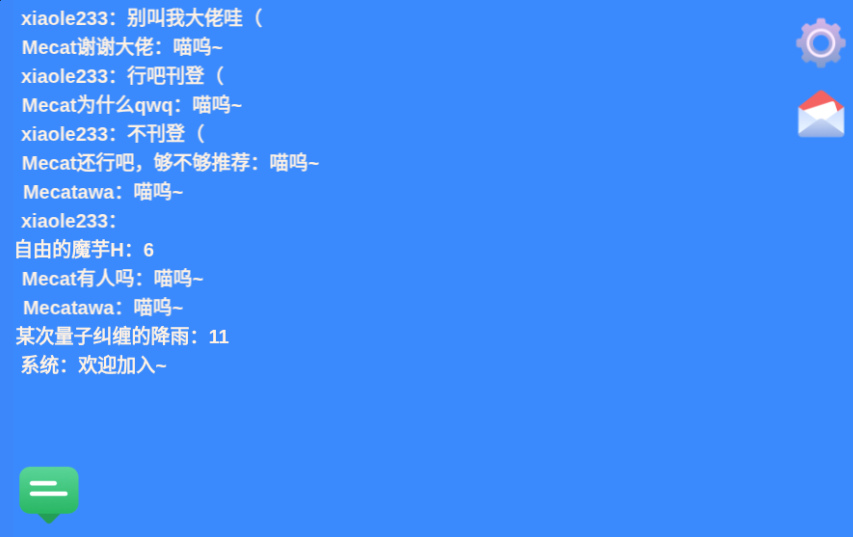
\includegraphics[width=0.5\textwidth]{assets/01/kitten-1.png}

\noindent
\textbf{作者:} \\
\textbf{ID:} \\
\textbf{介绍:} \\
\textbf{编辑评:}
\hfill
\includegraphics[width=0.08\columnwidth]{assets/01/kitten-1-qrc.png}
\subsection{作品B}
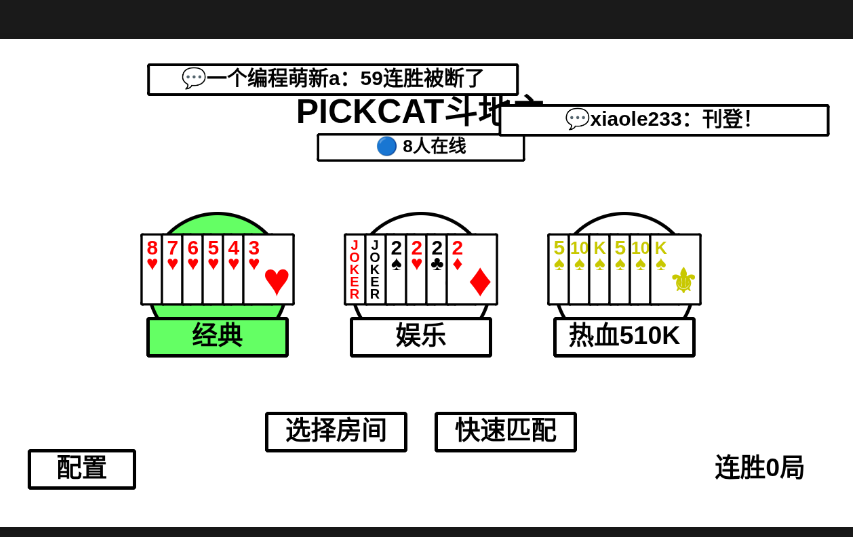
\includegraphics[width=0.5\textwidth]{assets/01/kitten-2.png}

\noindent
\textbf{作者:} \\
\textbf{ID:} \\
\textbf{介绍:}\\
\textbf{编辑评:}
\hfill
\includegraphics[width=0.08\columnwidth]{assets/01/kitten-2-qrc.png}

\pagebreak
\part{代码诗篇}
\subsection{作品A}
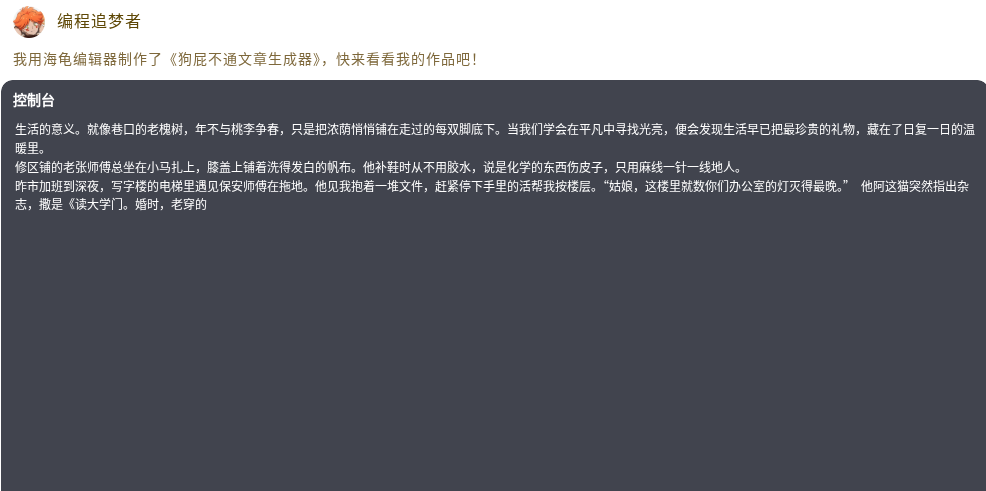
\includegraphics[width=0.5\textwidth]{assets/01/python-1.png}

\noindent
\textbf{作者:} \\
\textbf{链接:}https://shequ.codemao.cn/community/1632113 \\
\textbf{介绍:}\\
\textbf{编辑评:}
\hfill 
\includegraphics[width=0.08\columnwidth]{assets/01/python-1-qrc.png}

\subsection{作品B}
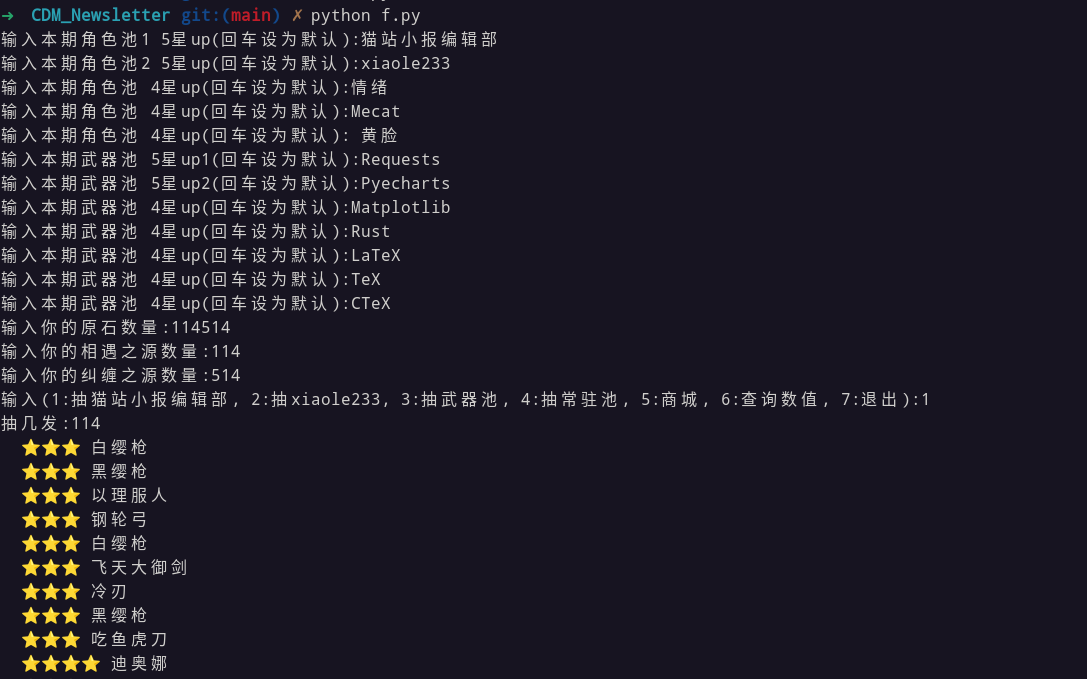
\includegraphics[width=0.4\textwidth]{assets/02/python-2.png}

\noindent
\textbf{作者:}不知名的原神玩家 \\
\textbf{Github仓库地址:} \\
\textbf{介绍:}一个用Python写的原神抽卡模拟器,代码量600多行\\
\textbf{编辑评:}编辑部已放弃重构
\hfill 
\includegraphics[width=0.08\columnwidth]{assets/02/python-2-qrc.png}

\pagebreak
\part{传火者}
\begin{center}
	\zihao{-1}
	\textbf{标题}
	\normalsize
	供稿:
\end{center}


\part{后记}
\paragraph{编辑} 目前唯一编辑也是主笔:xiaole233 邮箱地址:xiao\_2010@outlook.com
\paragraph{版权说明} 刊登的所有作品及文章均以取得原作者同意。\\ 
猫站小报 第一期  © 2025 by 小报编辑部 is licensed under CC BY 4.0.\\ To view a copy of this license, visit https://creativecommons.org/licenses/by/4.0/

\end{document}